\section{Fraud management cycle}
    This reasoning comes directly from every single step we analised in the previous section.
    The fraud management cycle is composed by the following parts:
    \begin{figure}[ht!]
        \centering
        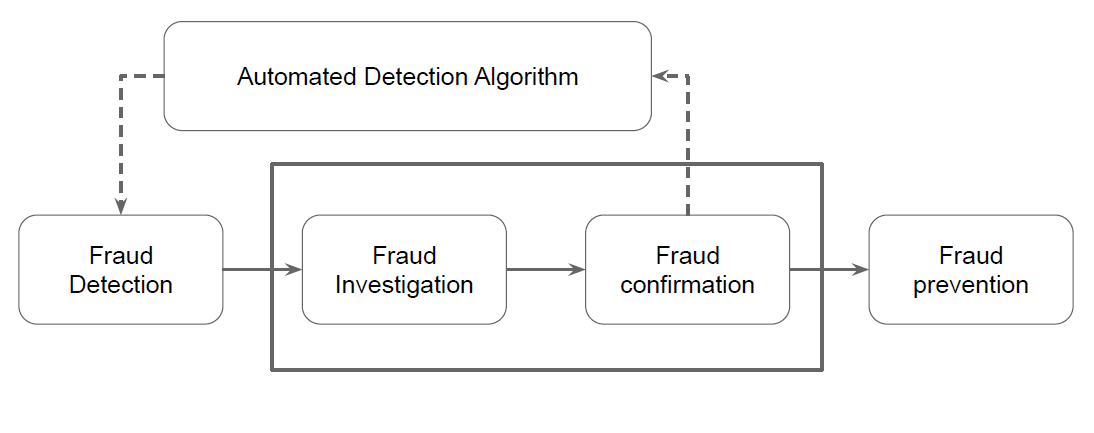
\includegraphics[width=0.6\linewidth]{cycle.png}
    \end{figure}
    \begin{itemize}
        \item \textbf{Fraud Detection:} Applying detection models on new, unseen observations and assigning a fraud risk to every observation
        \item \textbf{Fraud Investigation:} A human expert investigates suspicious, flagged cases given the involved subtlety and complexity
        \item \textbf{Fraud Confirmation:} Determining true fraud label, possibly involving field research
        \item \textbf{Fraud Prevention:} Preventing fraud to be committed in the future
        \item \textbf{Automated Detection Algorithm:} Feedback loop: newly detected cases should be added to the database of historical fraud cases, used to learn or induce the detection model
    \end{itemize}
    \subsection{Regular update of the model}
        A regular update is recommendable given the dynamic nature of fraud.\\
        With which frequency should the model be retrained or updated? It depends on several factors:
        \begin{itemize}
            \item The volatility of the fraud behavior
            \item The detection power of the current model
            \item The amount of confirmed cases already available in the database
            \item The rate at which new cases are being confirmed 
            \item The required effort to retrain the model
        \end{itemize}
        The model must be monitored to verify its performances day by day.
\section{Fraud Analytical Process}
    If you want to build a data driven model you have to follow a sequence of steps that are part of an iterative model:
    \begin{figure}[ht!]
        \centering
        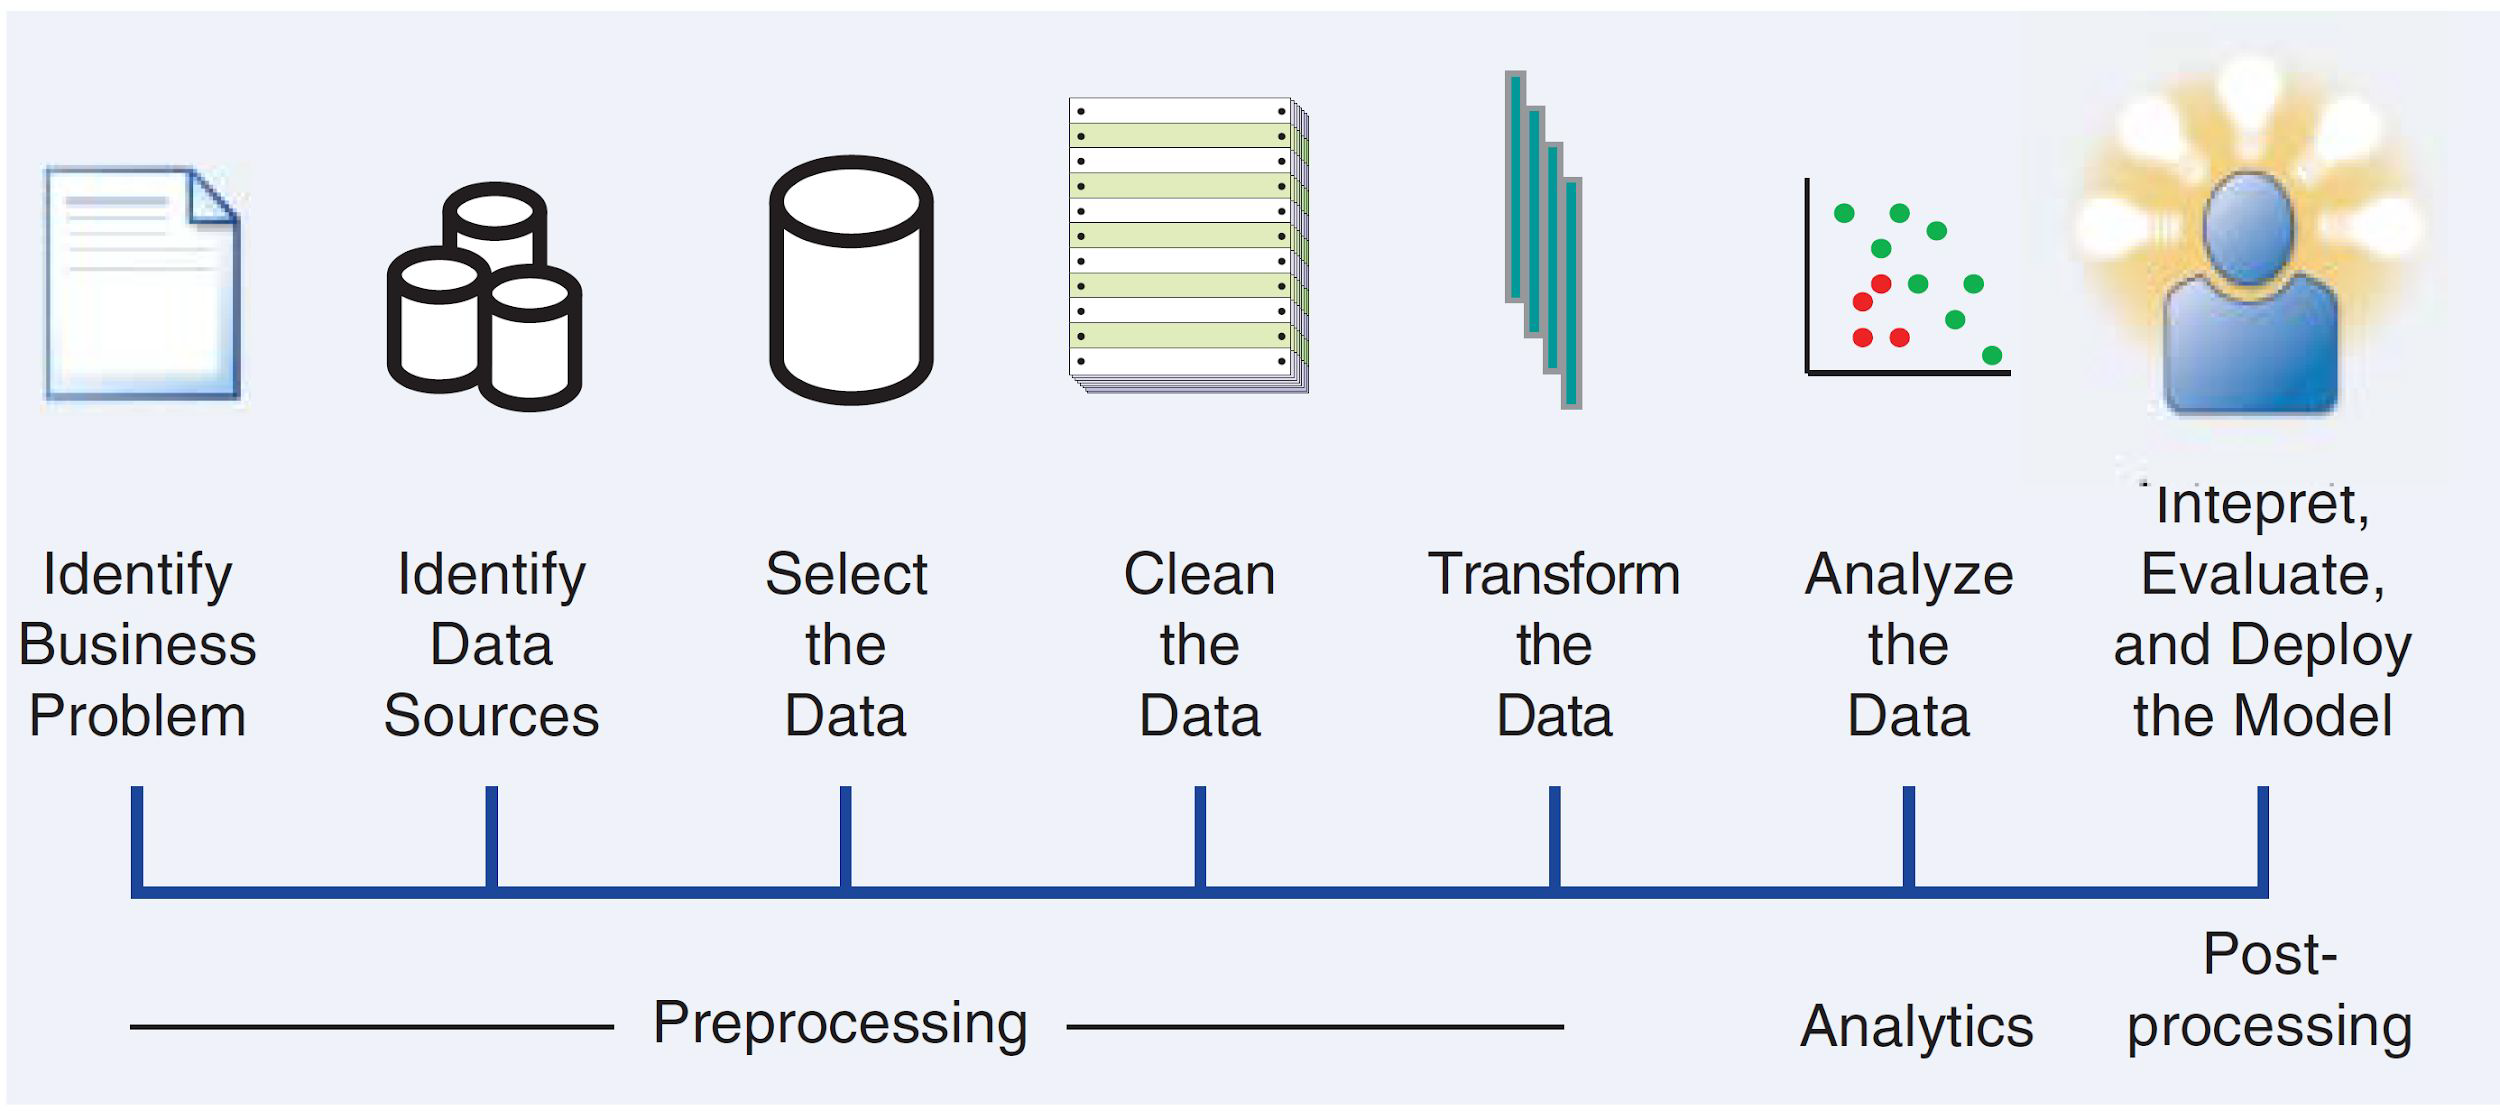
\includegraphics[width=0.6\linewidth]{process.png}
    \end{figure}
    \textbf{The preprocessing part is always an important and crytical part}:
    \begin{itemize}
        \item \textbf{Identify business problem}
        \item \textbf{Identify data sources:} data are the key ingredient to any analytical exercise
        \item \textbf{Select the data:} data selection has an impact on the analytical models
        \item \textbf{Clean the data:} get rid of inconsistencies, such as missing values and duplicate data 
        \item \textbf{Transform the data:} additional transformations
    \end{itemize}
    \textbf{Analytics:} the analytical model is estimated on the preprocessed and transformed data. The actual fraud-detection model is built\\
    \textbf{Post-processing:} the model is interpreted and evaluated by the fraud experts
    \subsection{Possible analysis output}
        When we build a model we want it to be able to:
        \begin{itemize}
            \item Be able to confirm and detect the same fraud present in the dataset: \textbf{trivial fraudulent patterns}
            \item Be able to detect novel knowledge, it must be able to generalise: \textbf{unknown patterns}
        \end{itemize}
        Once the analytical model has been appropriately validated and approved, it can be put into production
    \subsection{Additional consideration}
        Each alerted fraud must be investigated: the output of the model must be user-friendly.\\
        To be in \textit{the pipeline}, the model has to be integrated with other applications, part of the company system.\\
        The model must be also monitored and updated on a regular basis 
    \subsection{Key characteristics of a successful fraud analytics model}
        \subsubsection{Statistical accuracy}
            We need to make sure that the model besides being very good at detecting frauds in the train environment, it must be able to generalise well and not overfitting.
        \subsubsection{Interpretability}
            When a deeper understanding of the detected frauds is required, a fraud-detection model must be interpretable. Model's interpretability depends on the technique used:
            \begin{itemize}
                \item \textbf{Open-box models:} it is possible to understand the underlying reasons why the model signals a case to be suspicious
                \item \textbf{Closed-box models:} non interpretable models
            \end{itemize}
        \subsubsection{Operational efficiency}
            When cases need to be evaluated in real time, operational efficiency is crucial and is a main concern during model performance assesment.
        \subsubsection{Fraud Detection Costs}
            Developing and implementing a fraud-detection model involves a significant cost to an organization.\\
            Cost-benefit analysis to gain insight of the returns on investment of building an advanced fraud-detection system:
            \begin{itemize}
                \item \textbf{Direct costs:}
                \begin{itemize}
                    \item Management
                    \item Operational
                    \item Equipment
                \end{itemize}
                \item \textbf{Indirect costs (more relevant):}
                \begin{itemize}
                    \item Less usability
                    \item Slower performance
                    \item Less privacy (due to security controls)
                    \item Reduced productivity (slower users)
                \end{itemize}
            \end{itemize}
            More money doesn't always mean more security.
        \subsubsection{Regulatory compliance}
            Depending on the context there may be internal or organization specifica and external regulation that applies to the development and application of a model, \textbf{a fraud-detection model should be in line and comply with all applicable regulation and legislation} 